\documentclass[titlepage,a4paper]{article}

\usepackage{xcolor}
\usepackage{a4wide}
\usepackage[colorlinks=true,linkcolor=black,urlcolor=blue,bookmarksopen=true]{hyperref}
\usepackage{bookmark}
\usepackage{fancyhdr}
\usepackage[spanish]{babel}
\usepackage[utf8]{inputenc}
\usepackage[T1]{fontenc}
\usepackage{listings}
\usepackage{graphicx}
\usepackage{float}
\usepackage{hyperref}
\pagestyle{fancy} % Encabezado y pie de página
\fancyhf{}
\fancyhead[L]{Ejercicios de Parcial}
\fancyhead[R]{Introducción a Sistemas Distribuidos - FIUBA}
\renewcommand{\headrulewidth}{0.4pt}
\fancyfoot[C]{\thepage}
\renewcommand{\footrulewidth}{0.4pt}



% code listing settings
\usepackage{listings}
\renewcommand{\lstlistingname}{Código \textnumero{}}
\lstset{
    language=Python,
    basicstyle=\ttfamily\small,
    aboveskip={1.0\baselineskip},
    belowskip={1.0\baselineskip},
    columns=fixed,
    extendedchars=true,
    breaklines=true,
    tabsize=4,
    prebreak=\raisebox{0ex}[0ex][0ex]{\ensuremath{\hookleftarrow}},
    frame=lines,
    showtabs=false,
    showspaces=false,
    showstringspaces=false,
    keywordstyle=\color[rgb]{0.627,0.126,0.941},
    commentstyle=\color[rgb]{0.133,0.545,0.133},
    stringstyle=\color[rgb]{01,0,0},
    numbers=left,
    numberstyle=\small,
    stepnumber=1,
    numbersep=10pt,
    captionpos=t,
    escapeinside={\%*}{*)}
}


\begin{document}
\begin{titlepage} % Carátula
	\hfill
\includegraphics[width=6cm]{imagenes/logofiuba.jpg}
    \centering
    \vfill
    \Huge \textbf{Resumen parcial}
    \vskip2cm
    \Large [75.43]  Introducción Sistemas Distribuidos\\
    Curso Hamelin \\ 
    Primer cuatrimestre de 2022 
    \vfill
    \begin{tabular}{ | l | l | } % Datos del alumno
      \hline
      VAZQUEZ LAREU, Román & 100815 \\ \hline
      

  	\end{tabular}
    \vfill
    \vfill
\end{titlepage}

\tableofcontents % Índice general
\newpage

\section{Calcular RTT}\label{sec:CalcularRTT}

\textbf{Tiempo de inserción}: tiempo que tarda el paquete en ser insertado en el enlace

$$t_{ins} = \frac{L}{R}$$ 

\begin{itemize}
    \item $L$: largo del paquete
    \item $R$: velocidad de serialización
\end{itemize}


\textbf{Tiempo de propagación}: Tiempo que demora el paquete en propagarse por el enlace de un router al próximo

$$t_{prop} = \frac{d}{c}$$

\begin{itemize}
    \item $d$: distancia entre extremos del enlace
    \item $c$: velocidad del medio
        \subitem Aire: $c = 3x10^8 \frac{m}{s}$
        \subitem Fibra, cobre,etc: $\frac{2}{3} c$ 
\end{itemize}


\textbf{Qué tiempo es más influyente?}
\begin{itemize}
    \item Distancias largas: $ t_{ins} <  t_{prop} $
    \item Distancias cortas: $ t_{ins} > t_{prop}$
\end{itemize}





\begin{figure}[H]
\centering
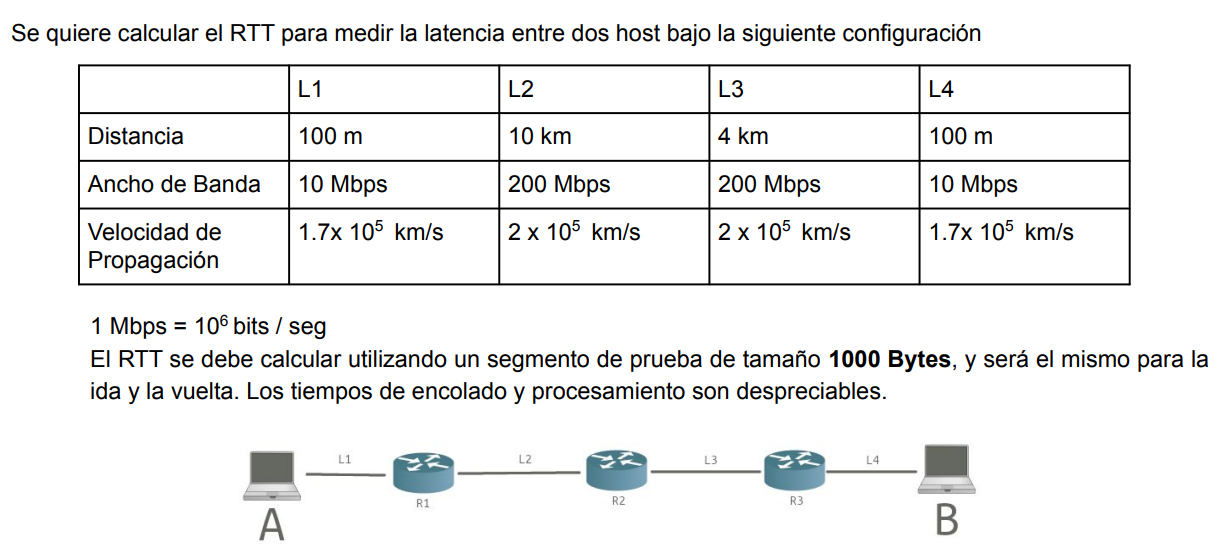
\includegraphics[width=\textwidth]{imagenes/ejercicioRtt.png}
\end{figure}


RTT o Round-Trip-Time es el tiempo que tarda un paquete de datos enviado desde un emisor en volver
al mismo emisor habiendo pasado por el receptor de destino.

Al tener las velocidades de propagación en $\frac{Km}{s}$, se pasan las distancias a $Km$

$$D_{L1} = 100 m = 0.1 \; Km$$
$$D_{L2} = 10 \; Km$$
$$D_{L3} = 4 \; Km$$
$$D_{L4} = 100 m = 0.1 \; Km$$

Se pasa el ancho de banda a $bits/seg$

$$t_{ins1} = 10 Mbps = 10^7 \frac{bits}{seg}$$
$$t_{ins2} = 200 Mbps = 20\cdot 10^7 \frac{bits}{seg}$$
$$t_{ins3} = 200 Mbps = 20\cdot 10^7 \frac{bits}{seg}$$
$$t_{ins4} = 10 Mbps = 10^7 \frac{bits}{seg}$$

Largo del paquete a $bits$

$$1000 \; bytes = 8000 \; bits$$

\textbf{Análisis tiempo de inserción}: \\


\begin{figure}[H]
\centering
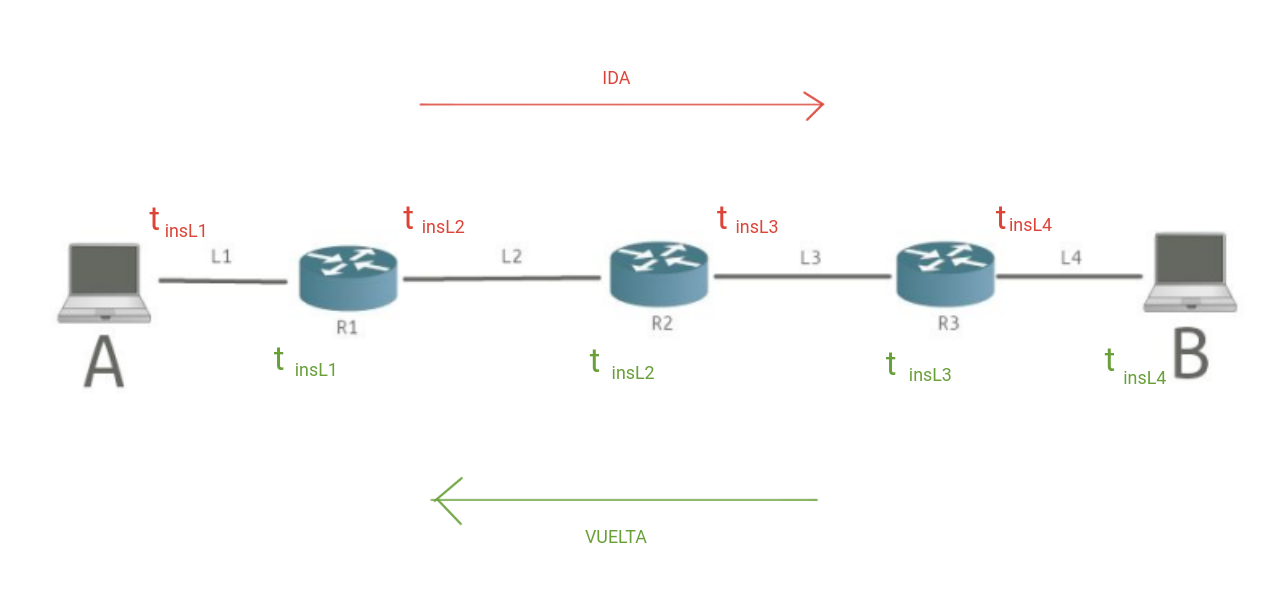
\includegraphics[width=\textwidth]{imagenes/tiempoInsercion.png}
\end{figure}



Ida:

$$ t_{insIDA} = t_{insL1} + t_{insL2} + t_{insL3} +t_{insL4} $$ 
$$\frac{8000 bits}{10^7 \frac{bits}{seg}}  + \frac{8000 bits}{20\cdot 10^7 \frac{bits}{seg}}  + \frac{8000 bits}{20\cdot 10^7 \frac{bits}{seg}} + \frac{8000 bits}{10^7 \frac{bits}{seg}} = 1.68 \cdot 10^-3 seg$$

Vuelta:

$$ t_{insVUELTA} = t_{insL4} + t_{insL3} + t_{insL2} +t_{insL1} $$ 
$$  \frac{8000 bits}{10^7 \frac{bits}{seg}}  + \frac{8000 bits}{20\cdot 10^7 \frac{bits}{seg}}  + \frac{8000 bits}{20\cdot 10^7 \frac{bits}{seg}} + \frac{8000 bits}{10^7 \frac{bits}{seg}} = 1.68 \cdot 10^{-3} seg $$

Total:

$$ t_{ins} = t_{insIDA} + t_{insVUELTA} =   1.68 \cdot 10^{-3} seg +  1.68 \cdot 10^{-3} seg =  3.36 \cdot 10^{-3} \; seg$$


\textbf{Análisis tiempo de propagación}: \\

\begin{figure}[H]
\centering
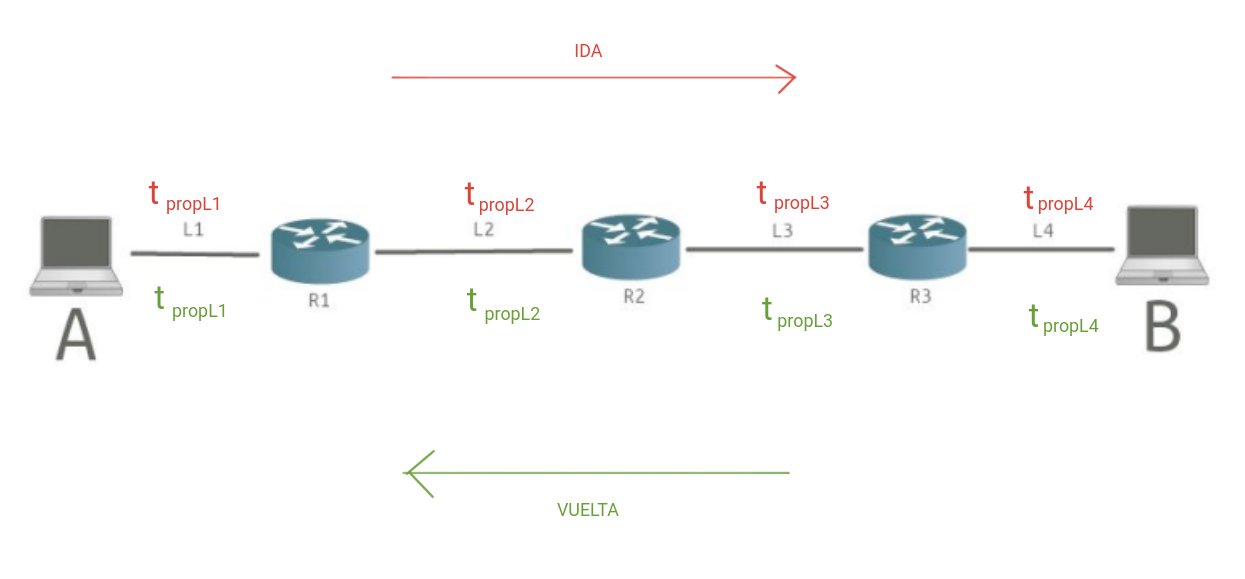
\includegraphics[width=\textwidth]{imagenes/tiempoPropagacion.png}
\end{figure}

Ida:

$$t_{propIDA} = t_{propL1} + t_{propL2}  + t_{propL3} + t_{propL4} $$ 
$$ \frac{0.1 \; Km}{1.7\cdot10^5\frac{Km}{seg}} + \frac{10 \; Km}{2\cdot10^5\frac{Km}{seg}} + \frac{4 \; Km}{2\cdot10^5\frac{Km}{seg}} + \frac{0.1 \; Km}{1.7\cdot10^5\frac{Km}{seg}} = 7.11765 \cdot 10^{-5} \; seg $$

Vuelta:

$$t_{propVUELTA} = t_{propL4} + t_{propL3} + t_{propL2} + t_{propL1} $$ 
$$ \frac{0.1 \; Km}{1.7\cdot10^5\frac{Km}{seg}} + \frac{10 \; Km}{2\cdot10^5\frac{Km}{seg}} + \frac{4 \; Km}{2\cdot10^5\frac{Km}{seg}} + \frac{0.1 \; Km}{1.7\cdot10^5\frac{Km}{seg}} = 7.11765 \cdot 10^{-5} \; seg  $$

Total:

$$t_{prop} = t_{propIDA} + t_{propVUELTA}  =  7.11765 \cdot 10^{-5} \; seg + 7.11765 \cdot 10^{-5} \; seg = 1.42353\cdot10^{-4} \; seg$$

\textbf{Resolución final}:

$$ t_{prop} + t_{ins} = 1.42353\cdot10^{-4} \; seg + 3.36 \cdot 10^{-3} \; seg = 3.50235 \cdot 10^{-3} \; seg$$

$$ RTT = 3.5 \; ms$$


\subsection{Otros}

\textbf{Tiempo de procesamiento}: es el tiempo que requiere el procesamiento del paquete en los routers. Implica leer el header y tomar la decisión de por cuál enlace enviarlo. Los órdenes de tiempo se encuentran entre los nano y microsegundos ($ns$, $\mu s$ )

\textbf{Tiempo de encolado}: es el tiempo que espera paquete en el router desde que arriba hasta que es finalmente transmitido. Depende de la tasa de desocupación del router, del tamaño de la cola. A mayor tráfico, mayor tiempo encolado. Este tiempo no es constante sino aleatorio, varía con el tráfico

\begin{figure}[H]
\centering
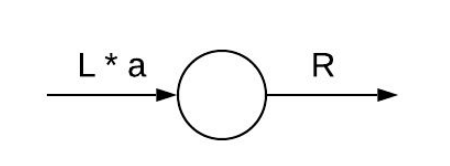
\includegraphics[width=\textwidth]{imagenes/tiempoEncolado.png}
\caption{Tiempo de Encolado}
\end{figure}

\begin{itemize}
    \item L: largo del paquete
    \item a: tasa de arribo promedio de paquete
    \item R: velocidad de serialización
\end{itemize}

Si $L \cdot a > R$, significa que están llegando más paquetes que los que el router puede procesar, se va llenando el buffer hasta estarlo por completo y comenzar a descartar paquetes. Si $L \cdot a = R$ la cola se llena, entonces la solución es la subutilización, es decir $L \cdot a < R$

\begin{figure}[H]
\centering
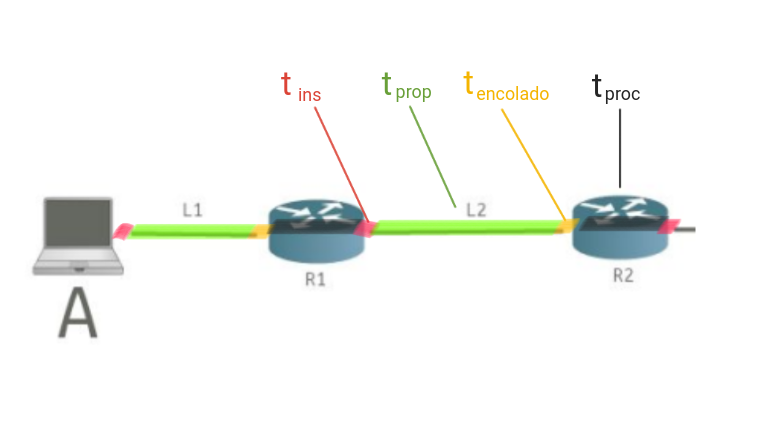
\includegraphics[width=\textwidth]{imagenes/tiemposRTT.png}
\caption{Tiempo de Encolado}
\end{figure}

\section{Agregación de prefijos}\label{sec:agrprefijos}

Permite reducir la cantidad de entradas en la tabla de ruteo. Puede realizarse cuando \textbf{las redes son contiguas} y cuando tienen \textbf{idéntico Next Hop o puerto de salida}. Se dice que dos redes son contiguas cuando tienen \textbf{prefijos de igual longitud} y \textbf{la máscara sólo difiere en el último bit}


\subsection{Caso Favorable}

\begin{center}
    \begin{tabular}{c|c}
        Máscara & Puerto de salida \\
        \hline
        \hline
         192.168.0.0/24 &  0\\
         \hline
         192.168.1.0/24 &  0
    \end{tabular}
\end{center}

El \textbf{/24} indica que deben tomarse los primeros 24 bits
Si pasamos a binario:

\begin{center}
    \begin{tabular}{c|c|c|c}
        0-7 bits & 8-14 bits & 15-23 bits & 24-31 bits \\
        \hline
        \hline
        192 & 168 & 0000000 \textbf{0} & 00000000 \\
        \hline
        192 & 168 & 0000000 \textbf{1} & 00000000 \\
    \end{tabular}
\end{center}

Difieren sólo en el último bit (el bit número 24) y el prefijo es de igual longitud, por lo que son contiguas. Además tienen el mismo puerto de salida. Se puede hacer agregación de prefijos

\begin{center}
    \begin{tabular}{c|c}
        Máscara & Puerto de salida \\
        \hline
        \hline
         192.168.0.\textbf{0/23} &  0\\
    \end{tabular}
\end{center}

Se disminuyó en uno la máscara y se las unificó en una sola red

\subsection{Caso Desfavorable por no ser contiguas - bit}

\begin{center}
    \begin{tabular}{c|c}
        Máscara & Puerto de salida \\
        \hline
        \hline
         192.168.1.0/24 &  0\\
         \hline
         192.168.2.0/24 &  0
    \end{tabular}
\end{center}

El \textbf{/24} indica que deben tomarse los primeros 24 bits
Si pasamos a binario:

\begin{center}
    \begin{tabular}{c|c|c|c}
        0-7 bits & 8-14 bits & 15-23 bits & 24-31 bits \\
        \hline
        \hline
        192 & 168 & 000000 \textbf{01} & 00000000 \\
        \hline
        192 & 168 & 000000 \textbf{10} & 00000000 \\
    \end{tabular}
\end{center}

No difieren únicamente en el último bit, por lo que no cumplen con ser contiguas, por lo que no se puede realizar agregación de prefijos


\subsection{Caso Desfavorable por no ser contiguas - Next Hop}

\begin{center}
    \begin{tabular}{c|c}
        Máscara & Puerto de salida \\
        \hline
        \hline
         192.168.0.0/24 &  \textbf{0}\\
         \hline
         192.168.1.0/24 &  \textbf{1}
    \end{tabular}
\end{center}

Si bien son contiguas, al no compartir el next hop, no se puede realizar agregación de prefijos


\subsection{Ejercicio de parcial}

Simplificar la siguiente tabla

\begin{center}
    \begin{tabular}{c|c}
        Máscara & Puerto de salida \\
        \hline
        \hline
        157.128.2.0/23 &  0\\
        \hline
        168.123.0.0/24 &  1 \\
        \hline
        168.123.1.0/24 &  1 \\
        \hline
        168.12.128.0/19 &  2 \\
        \hline
        168.12.160.0/19 &  2 \\
    \end{tabular}
\end{center}


Únicamente se podrá hacer agregación en aquellas que tengan igual puerto de salida, serán las que se analizarán.
Se analizan las del puerto de salida 1

\begin{center}
    
    \begin{tabular}{c|c|c|c}

        0-7 bits & 8-14 bits & 15-23 bits & 24-31 bits \\
        \hline
        \hline
        168 & 123 & 0000000 \textbf{0} & 00000000 \\
        \hline
        168 & 123 & 0000000 \textbf{1} & 00000000 \\
    \end{tabular}
\end{center}


Difieren en el último bit, el prefijo es de igual longitud y el mismo puerto de salida. Realizo agregación de prefijos.


\begin{center}
    \begin{tabular}{c|c}
        Máscara & Puerto de salida \\
        \hline
        \hline
        168.123.0.0/23 &  1 \\
    \end{tabular}
\end{center}

Se analizan las del puerto de salida 2

\begin{center}
    \begin{tabular}{c|c|c|c}
        0-7 bits & 8-14 bits & 15-23 bits & 24-31 bits \\
        \hline
        \hline
        168 & 12 & 10\textbf{0} 00001 & 00000000 \\
        \hline
        168 & 12 & 10\textbf{1} 00000 & 00000000 \\
    \end{tabular}
\end{center}

Difieren en el último bit, el prefijo es de igual longitud y el mismo puerto de salida. Realizo agregación de prefijos 

\begin{center}
    \begin{tabular}{c|c}
        Máscara & Puerto de salida \\
        \hline
        \hline
        168.12.128.0/18 &  2 \\
    \end{tabular}
\end{center}

Tabla final simplificada

\begin{center}
    \begin{tabular}{c|c}
        Máscara & Puerto de salida \\
        \hline
        \hline
        157.128.2.0/23 &  0\\
        \hline
        168.123.0.0/23 &  1 \\
        \hline
        168.12.128.0/18 &  2 \\
    \end{tabular}
\end{center}



\section{Control de flujo y congestion}

Cada extremo de la transmisión TCP tiene su propio buffer, alli almacena datos TCP para pasarlos a la capa de aplicación. Si se reciben más datos de los que la capa de aplicación es capaz de consumir, ocurre un \textit{buffer overflow}. Para evitar esto, cada extremo comunica la cantidad de datos que puede recibir. A esto se lo llama \textbf{rwnd} o \textit{Receiver Window}. Va en el campo \textit{Window} del header de TCP.
Cuando se recibe un cambio en \textbf{rwnd}, el emisor debe modificar la tasa de envío para no provocar un \textit{buffer overflow} ni subutilizar el buffer. 
Si se recibe $\textbf{rwnd} = 0 $, el emisor debe dejar de enviar datos hasta recibir un nuevo valor de \textbf{rwnd}. Para recibir este nuevo valor, el emisor envía paquetes de 1 byte constantemente y el receptor responde con el tamaño de ventana. Cuando este tamaño ya no es cero, el emisor retoma el envio de datos.

La congestion es producto de múltiples flujos TCP en simultáneo sobre la misma red. Cunado se llena un buffer, se empiezan a descartar los segmentos. En estos casos se dice que la red está congestionada.

\textbf{cwnd} es la máxima cantidad de bytes que puede haber en vuelo.
$$ \mathrm{LastByteSent}-\mathrm{LastByteACKed} < \mathrm{min}(\mathrm{cwnd},\mathrm{rwnd}) $$


\subsection{Etapas en el control de congestion}

\begin{itemize}
    \item Slow Start
    \item Congestion avoidance
    \item Fast Retransmit
    \item Fast Recovery
\end{itemize}

\subsubsection{Slow Start}

$$\mathrm{cwnd}_{n+1} = \mathrm{cwnd_n} + \mathrm{MSS} \cdot \#\mathrm{ACK} $$

con \textbf{cwnd} medido en bytes


$$\mathrm{cwnd}_{n+1} = \mathrm{cwnd}_n + \#ACK $$

con \textbf{cwnd} medido en MSSs, es decir segmentos de tamaño máximo. Crece de manera exponencial. \\

\textbf{Ejemplo}



$$ \mathrm{cwnd}_0 = 1 $$

entonces envío 1 segmento, recibo 1 ACK. Luego 

$$ \mathrm{cwnd}_1 = \mathrm{cwnd}_0 + 1 = 1 + 1 = 2 $$

Envío entonces 2 segmentos, por los cuales recibo 2 ACKs

$$ \mathrm{cwnd}_2 = \mathrm{cwnd}_1 + \#ACK = 2 + 2 = 4 $$

Para frenar este crecimiento exponencial se cambia de etapa

\subsubsection{Congestion avoidance}

En un momento se da por terminada la etapa de slow start para pasar a la proximo, llamada congestion Avoidance. Esto viene dado por el valor \textbf{sstresh} o \textit{slow start threshold size}.

$$ \mathrm{cwnd}_{n+1} = \mathrm{cwnd}_n + \frac{\#ACK}{\mathrm{cwnd}_n} $$

Aumenta en 1 al llegar los ACKs de la ráfaga, cwnd \textbf{tiene que ser entero, la unidad es el MSS}. Llegado el caso, se redondea para abajo. \\

\textbf{Ejemplo}

$$\mathrm{cwnd}_n = 2$$

Entonces se envían 2 segmentos. Llega el primer ACK

$$ \mathrm{cwnd}_{n+1} = \mathrm{cwnd}_n +  \frac{\#ACK}{\mathrm{cwnd}_n} $$

$$ \mathrm{cwnd}_{n+1} = 2 +  \frac{1}{2} = 2.5 $$

$$ \mathrm{cwnd}_{n+1} = 2 $$

Llega el segundo ACK

$$ \mathrm{cwnd}_{n+2} = \mathrm{cwnd}_{n+1} +  \frac{\#ACK}{\mathrm{cwnd}_{n+1}} $$

$$ \mathrm{cwnd}_{n+2} = 2 +  \frac{2}{2} = 3 $$


\subsubsection{Pérdida de paquetes}

Pérdida por timeout (\textbf{RTO})

$$ \mathrm{ssthresh} = \frac{\mathrm{cwnd}_n}{2} $$

$$ \mathrm{cwnd}_{n+1} = 1  $$

1 es llamado LW o \textit{Loss Window}

\subsection{Ejercicio de parcial}



En una conexión TCP recién establecida (IW = 2 MSS, SSTHRESH = 64 KB) con RTT=200 ms y MSS=2 KB, el host receptor siempre anuncia una AdvertisedWindow de 16 KB. La red está cargada al punto que si una ráfaga fuera de 16 KB o más, se perderían todos los segmentos de la misma.
¿Cuántos rounds se demora en enviar un archivo
de 36 KB?



$$ \mathrm{RTT} = 200 ms $$

$$ \mathrm{MSS} = 2 KB$$

$$ IW = 2 MSS $$

$$ \mathrm{SSTHRESH} = 64 KB $$

$$ \mathrm{rwnd} = 16 KB $$

$$ \mathrm{LimiteDeLaRed} = 16 KB $$

$$ \mathrm{fileSize} = 36 KB $$

Paso los datos a MSS

$$ IW = 2 MSS $$

$$ \mathrm{SSTHRESH} = 32 MSS $$

$$ \mathrm{rwnd} = 8 MSS $$

$$ \mathrm{LimiteDeLaRed} = 8 MSS $$

$$ \mathrm{fileSize} = 18 MSS $$



\begin{figure}[H]
\centering
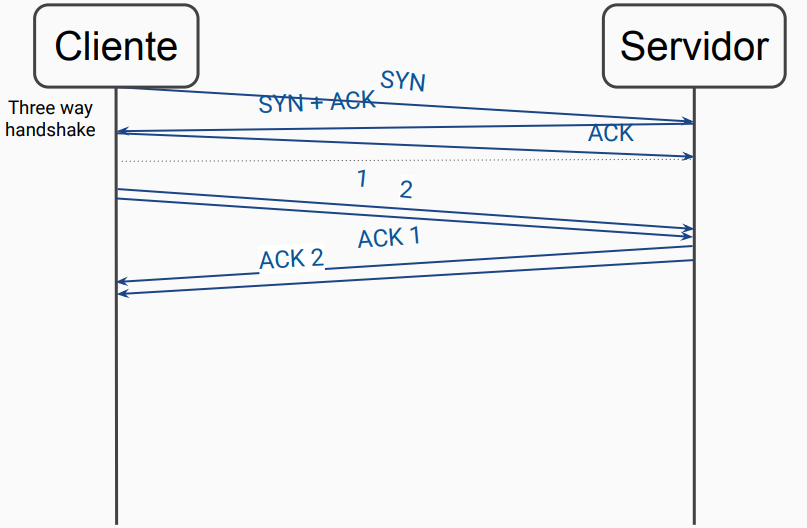
\includegraphics[width=\textwidth]{imagenes/resolucion1.png}
\end{figure}

En una primera instancia se realiza el three way handshake para establecer la conexion TCP. $IW = 2$ entonces $\mathrm{cwnd}_n = 2$. Se envían 2 segmentos, se reciben los 2 ACK correspondientes. Como se está en slow start, $$ \mathrm{cwnd}_{n+1} = \mathrm{cwnd}_n + \#ACK $$

De esta manera, $\mathrm{cwnd}_{n+1} = 2 + 2 = 4 $ y se envían 4 segmentos. De los cuales se reciben los 4 ACKs


\begin{figure}[H]
\centering
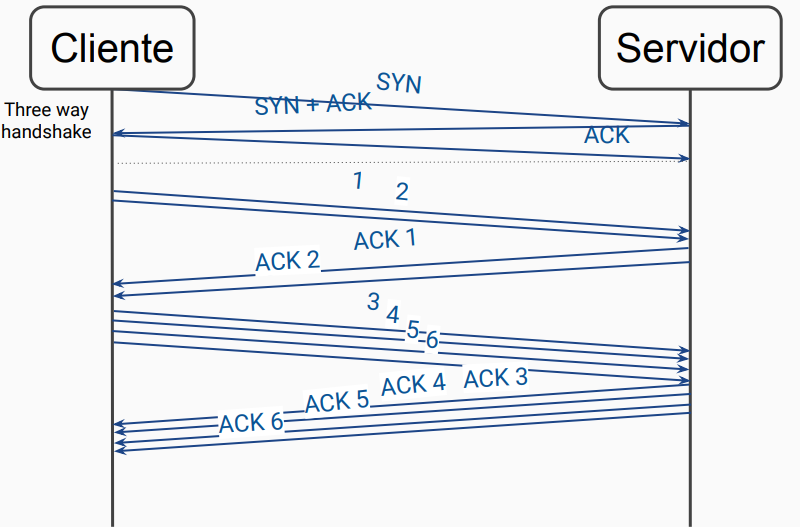
\includegraphics[width=\textwidth]{imagenes/resolucion2.png}
\end{figure}

se sigue en Slow start, por lo que  $\mathrm{cwnd}_{n+2} = \mathrm{cwnd}_{n+1} + \#\mathrm{ACK} = 4 + 4 = 8 $

Se envían entonces los siguientes 8 segmentos, los cuales se pierden ya que $ \mathrm{rwnd} = 8 $

\begin{figure}[H]
\centering
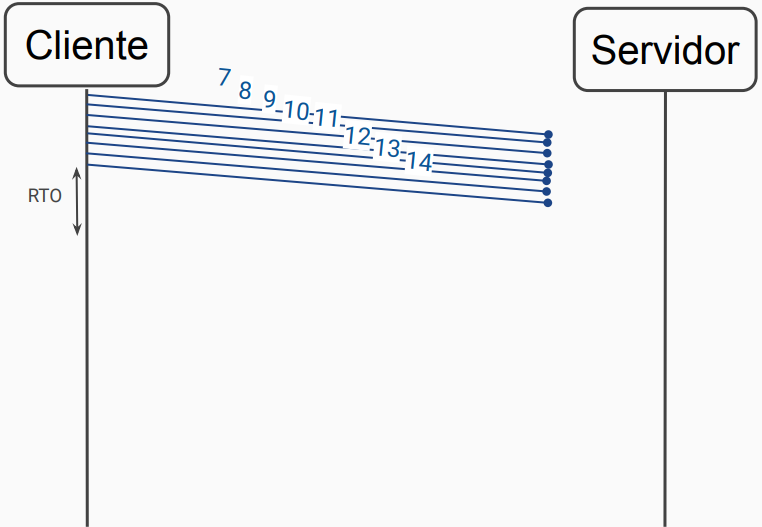
\includegraphics[width=\textwidth]{imagenes/resolucion3.png}
\end{figure}

El cliente se informa de esto por un timeout (RTO). Entonces debe actuarse teniendo en cuenta este evento. El valor de la ventana volverá a ser 1, por lo que $ \mathrm{cwnd}_{n+3} = 1  $. Además se modifica el threshold de acuerdo a $ \mathrm{ssthresh} = \frac{\mathrm{cwnd}_n}{2}  = \frac{8}{2} = 4$.

Se retoma entonces el envío de datos, enviando 1 segmento y recibiendo el ACK correspondiente. Se actualiza la ventana con $\mathrm{cwnd}_{n+4} = 1 +1 = 2$. Se envian entonces 2 y se reciben 2 ACK. Se llega a que $\mathrm{cwnd}_{n+5} = 2 + 2 = 4 $. 

\begin{figure}[H]
\centering
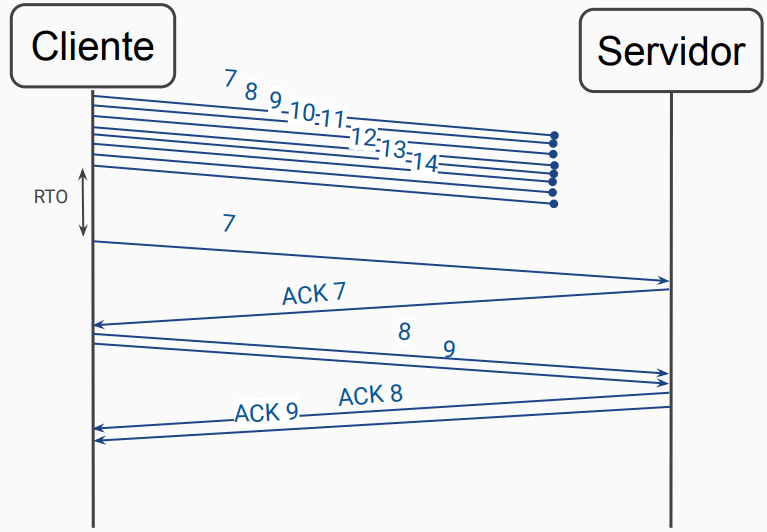
\includegraphics[width=\textwidth]{imagenes/resolucion4.png}
\end{figure}

Recordemos que por el RTO,  $ \mathrm{ssthresh} = 4 $, entonces $\mathrm{cwnd} \geq \mathrm{ssthresh} $. Entonces \textbf{finaliza Slow start y comienza congestion avoidance}.
Continuamos enviando 4 segmentos y recibimos los ACK correspondientes.
Ahora el cálculo de la ventana es distinto

$$ \mathrm{cwnd}_{n+1} = \mathrm{cwnd}_n + \frac{\#\mathrm{ACK}}{\mathrm{cwnd}_n} $$

entonces  $\mathrm{cwnd}_{n+6} = 4 + \frac{4}{4} = 5 $ y se envían 5 segmentos, de los cuales se reciben los 5 ACKs correspondientes. Ya se enviaron 18 MSS y como $\mathrm{fileName} = 18 \mathrm{MSS} $ es el fin de la transmisíon. 

\begin{figure}[H]
\centering
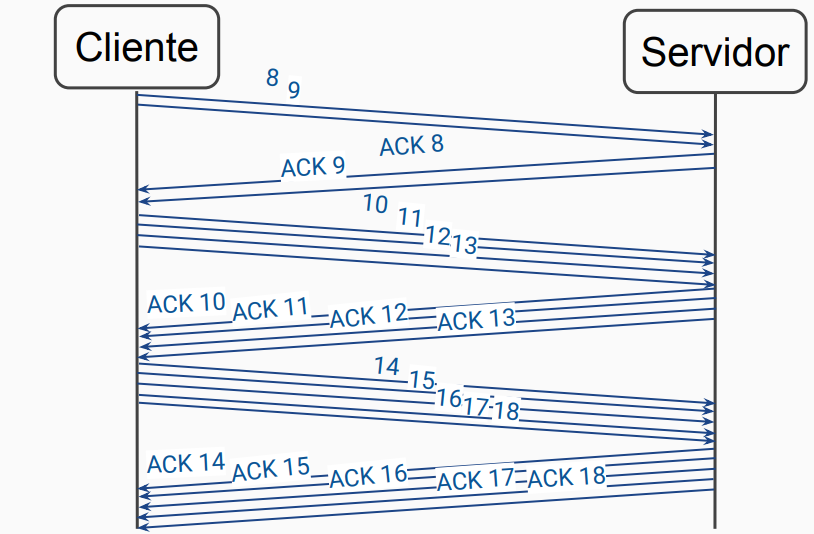
\includegraphics[width=\textwidth]{imagenes/resolucion5.png}
\end{figure}

Lo único que faltaría serian los mensajes correspondientes al cierre, que implica 4 mensajes

\begin{figure}[H]
\centering
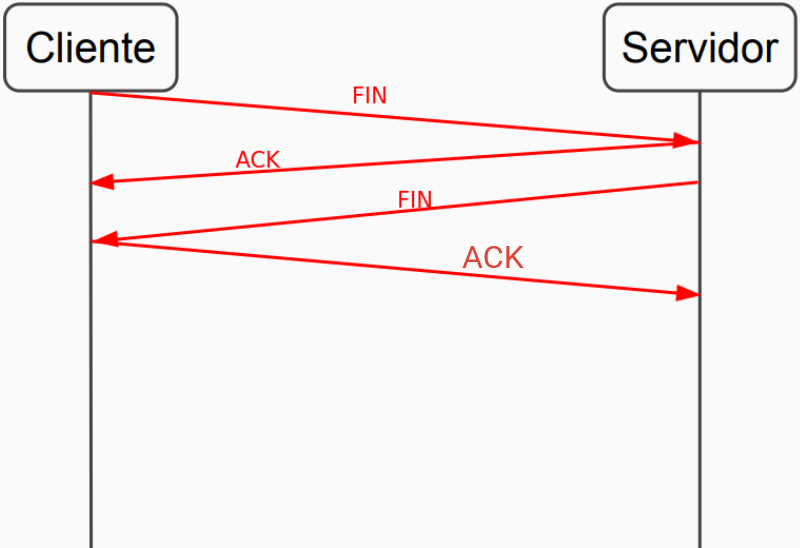
\includegraphics[width=\textwidth]{imagenes/resolucion6.png}
\end{figure}

\subsection{Pérdida de un solo paquete}

Suponemos se está usando el algoritmo de control de congestion de Tahoe. 
Recibib ACK duplicados indica que llegan algunos paquetes de la rafaga. Ocurre cuando se reciben 4 ACKs para el mismo segmento (el primer ACK es válido, luego llegan 3 ACKs duplicados). Dependiendo del algoritmo implementado se vuelve a slow start o se realiza un fast recovery

\subsubsection{Tahoe}

Tahoe se comporto frente a los ACKs duplicados de igual manera que lo hace frente a un RTO. Es decir, realiza un \textbf{Fast Retransmit} y luego un \textbf{Slow start} \\

\textbf{Ejemplo}\\

Veamos que ocurre cuando se pierde un paquete de una ráfaga con el algoritmo de Tahoe. El inicio de la comunicación es identico al caso anterior

\begin{figure}[H]
\centering
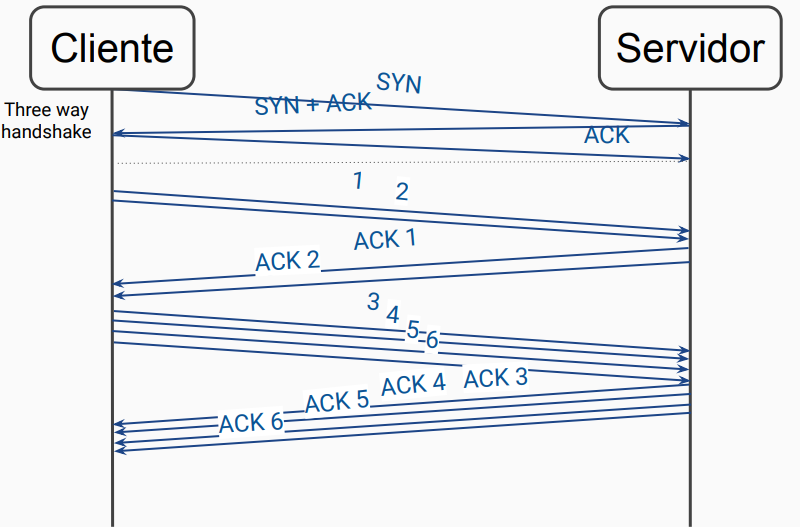
\includegraphics[width=\textwidth]{imagenes/resolucion2.png}
\end{figure}

En primer lugar el three Way Handshake, y los envios de paquetes van creciendo exponencialmente ya que nos encontramos en slow start. Luego de recibidos los ACK para los paquetes 3,4,5 y 6 el valor de la ventana es $\mathrm{cwnd}_n = 8$ y $\mathrm{ssthresh}  = 32$

En la siguiente ráfaga el paquete 8 no llega a destino, es decir llegan 7 paquetes al servidor. Por lo que este contesta con 7 ACK pero asociados al último paquete previo al que no llegó, es decir el paquete 7.

\begin{figure}[H]
\centering
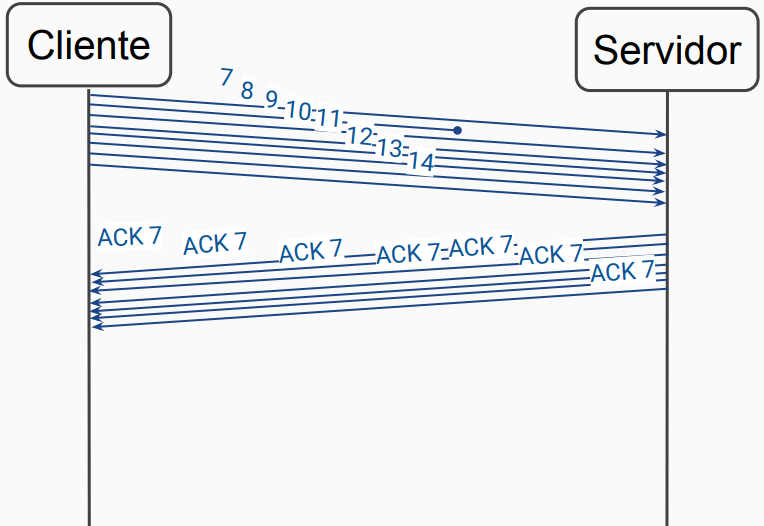
\includegraphics[width=\textwidth]{imagenes/paqEnRafaga.png}
\end{figure}


Al realizar esto el servidor, lo que está haciendo es un NACK implícito. Se ingresa entonces en \textbf{Fast Retransmit}, donde se envía el paquete extraviado y se recibe un ACK correspondiente al último paquete que se recibió correctamente de la ráfaga previa (el 14).


\begin{figure}[H]
\centering
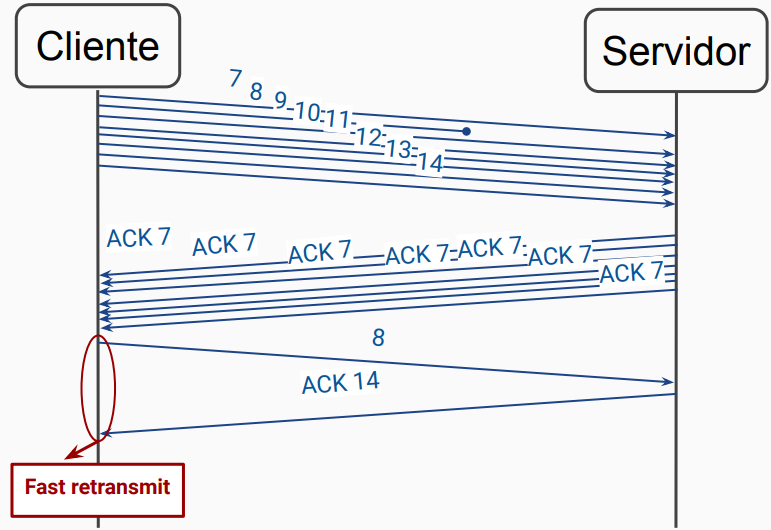
\includegraphics[width=\textwidth]{imagenes/fastRetransmit.png}
\end{figure}

Posterior a esto se vuelve a Slow Start, y Tahoe se comportaba de igual manera que en un RTO, por lo que $\mathrm{cwnd}_n = 1$ y $\mathrm{ssthresh} = \frac{\mathrm{cwnd}_{n-1}}{2} = \frac{8}{2} = 4 $. Entonces se envía un paquete y se recibe el ACK correspondiente. Luego se envían 2 y se reciben sus ACKs, etc


\subsubsection{Reno}

El algoritmo de Reno actúa distinto a Tahoe. Cuando se reciben 4 ACKs iguales, se retransmite el siguiente segmento. Además luego los valores son $ \mathrm{cwnd}_{n+1} = \frac{\mathrm{cwnd}_{n}}{2} $ y $ \mathrm{ssthresh} = \frac{\mathrm{cwnd}_{n}}{2} $. Luego de esto, se continúa en congestion Avoidance. Esto se llama \textbf{Fast Recovery} \\

\textbf{Ejemplo} \\

Identico al anterior hasta perder el 8vo paquete de la ráfaga. Se hace un fast retransmit del paquete perdido y se actualizan los valores de ventana y threshold. $\mathrm{cwnd}_n = 8 $ y $\mathrm{ssthresh} = 32$.

\begin{figure}[H]
\centering
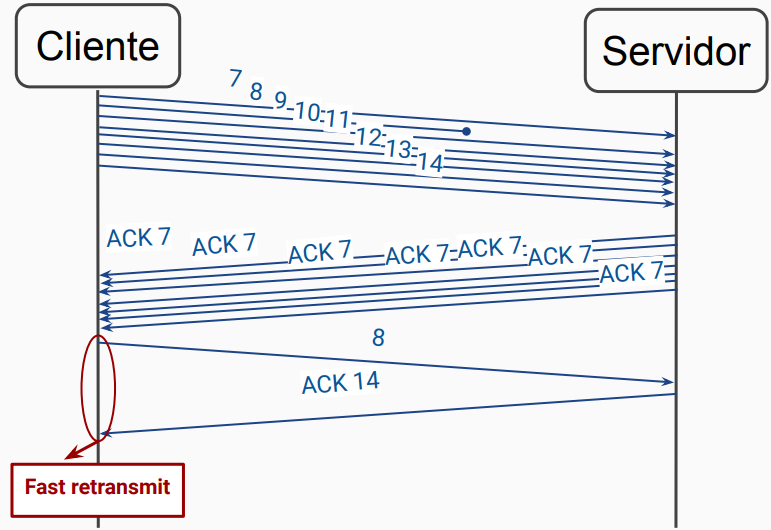
\includegraphics[width=\textwidth]{imagenes/fastRetransmit.png}
\end{figure}

Luego de reenviar el paquete perdido en fast retransmit,  $\mathrm{cwnd}_{n+1} = \frac{\mathrm{cwnd}_{n}}{2} = \frac{8}{2} = 4 $ y $\mathrm{ssthresh} = 4 $. A continuación se entra en congestion avoidance.

\begin{figure}[H]
\centering
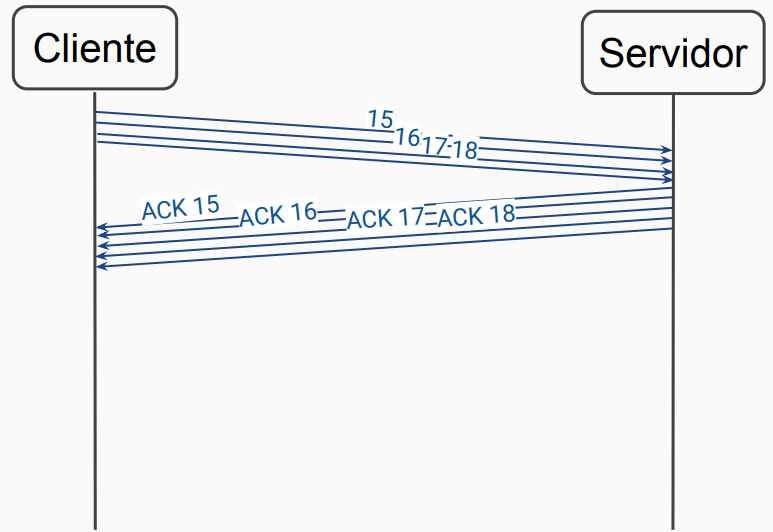
\includegraphics[width=\textwidth]{imagenes/postCongA.png}
\end{figure}

\subsubsection{Cheatsheet}

\textbf{En Slow Start}

$$ \mathrm{cwnd}_{n+1} = \mathrm{cwnd}_{n} + \#\mathrm{ACK} $$

\textbf{Ocurre RTO}

$$ \mathrm{ssthresh} = \frac{\mathrm{cwnd}_n}{2} $$

$$ \mathrm{cwnd}_{n+1} = 1  $$

\textbf{Congestion Avoidance, $\mathrm{cwnd} \geq \mathrm{ssthresh} $}

$$ \mathrm{cwnd}_{n+1} = \mathrm{cwnd}_n + \frac{\#\mathrm{ACK}}{\mathrm{cwnd}_n} $$


\subsection{Ejercicios de Parcial}

\subsubsection{Ejercicio 1}

Un usuario descarga un recurso de 30960 bytes de un servidor por medio de un HTTP GET. Se sabe que el sistema operativo del usuario opera con TCP Tahoe y cuya IW=4MSS. El sistema utiliza un ssthresh=11520 bytes. Considerando: 1MSS = 1440 bytes
La conexión sufrirá la pérdida del séptimo segmento de datos transmitido \\

Se que $ 1 \; \mathrm{MSS} = 1440 \; \mathrm{bytes} $ entonces se pasa todo a MSS. Para el recurso de $ 30960 \; \mathrm{bytes} $, $ \frac{30960 \; \mathrm{bytes} }{1440 \; \mathrm{bytes}} = 21.5 \; \mathrm{MSS}$. Como es el tamaño del archivo, para descargarlo por completo redondeo hacia arriba, entonces $ \mathrm{Recurso} = 22 \; \mathrm{MSS} $. Los mismo para $\mathrm{ssthresh}= 11520 \;\mathrm{bytes}$, entonces $\mathrm{ssthresh}= 8$. 
Como $\mathrm{IW} = 4 \; \mathrm{MSS}$ se comienza con $ \mathrm{cwnd}_n = 4$.



Primero el three way handshake para establecer la conexion TCP. Luego enviamos los primeros 4 paquetes y recibimos los 4 ACKs.


\begin{figure}[H]
\centering
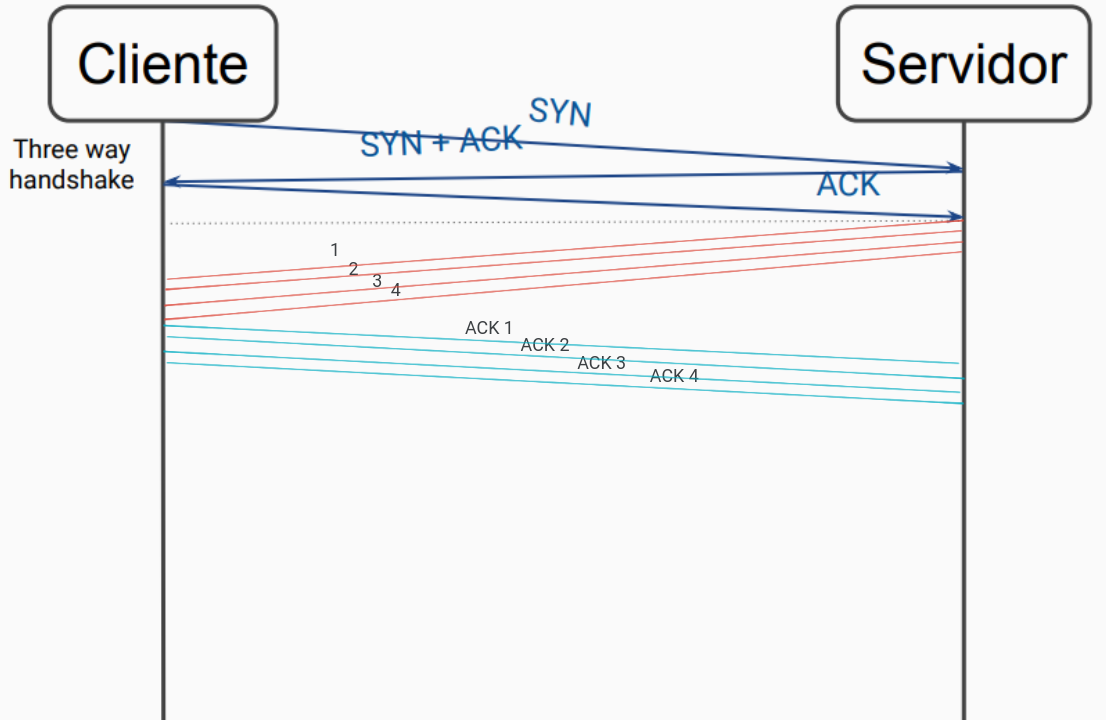
\includegraphics[width=\textwidth]{imagenes/resEj11.png}
\end{figure}

$ \mathrm{cwnd}_{n+1} = \mathrm{cwnd}_{n} + \#\mathrm{ACK} = 4 + 4 = 8 $. Se procede a enviar los siguientes 8 segmentos. Pero por consigna el 7mo no llega a destino. Por lo que se hace fast retransmit del segmento que no llega.

\begin{figure}[H]
\centering
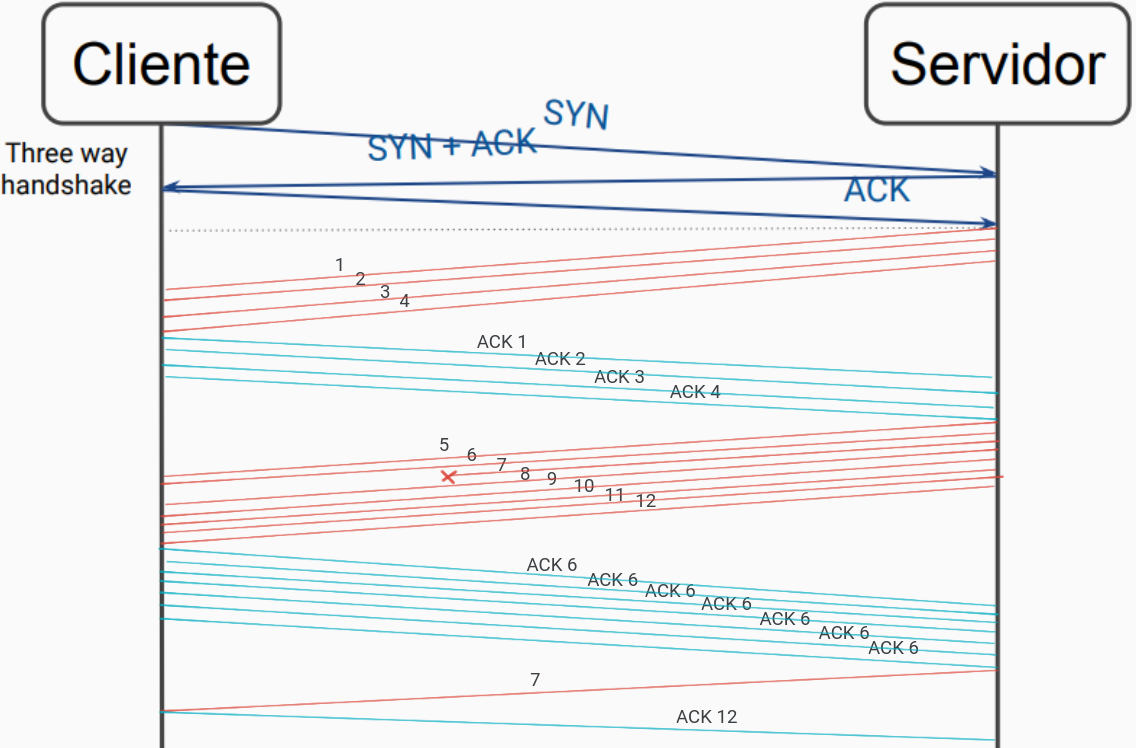
\includegraphics[width=\textwidth]{imagenes/resEj12.png}
\end{figure}

Como el algoritmo es Tahoe, posterior al Fast Retransmit, se vuelve a slow Start se tendrá $ \mathrm{cwnd}_{n+2} = 1 $ y   $\mathrm{ssthresh}= 4 $.

Se envía entonces un segmento, se recibe su ACK correspondiente. Por estar en Slow Start ahora  $ \mathrm{cwnd}_{n+3} = 2 $. Se envian 2 paquetes y se reciben los 2 ACKs. Ahora $ \mathrm{cwnd}_{n+4} = 4 $. Recordando que   $\mathrm{ssthresh}= 4 $, se envían 4 paquetes y se reciben los 4 ACK, pero ahora se actualiza distinto la ventana por haber entrado en Congestion Avoidance. $ \mathrm{cwnd}_{n+5} = \mathrm{cwnd}_{n+4} + \frac{\#\mathrm{ACK}}{\mathrm{cwnd}_{n+4}} = 4 + \frac{4}{4} = 5 $. 

Sin embargo, con enviar 3 paquetes más se completa la descarga del archivo. Se finaliza terminando la conexión.

\begin{figure}[H]
\centering
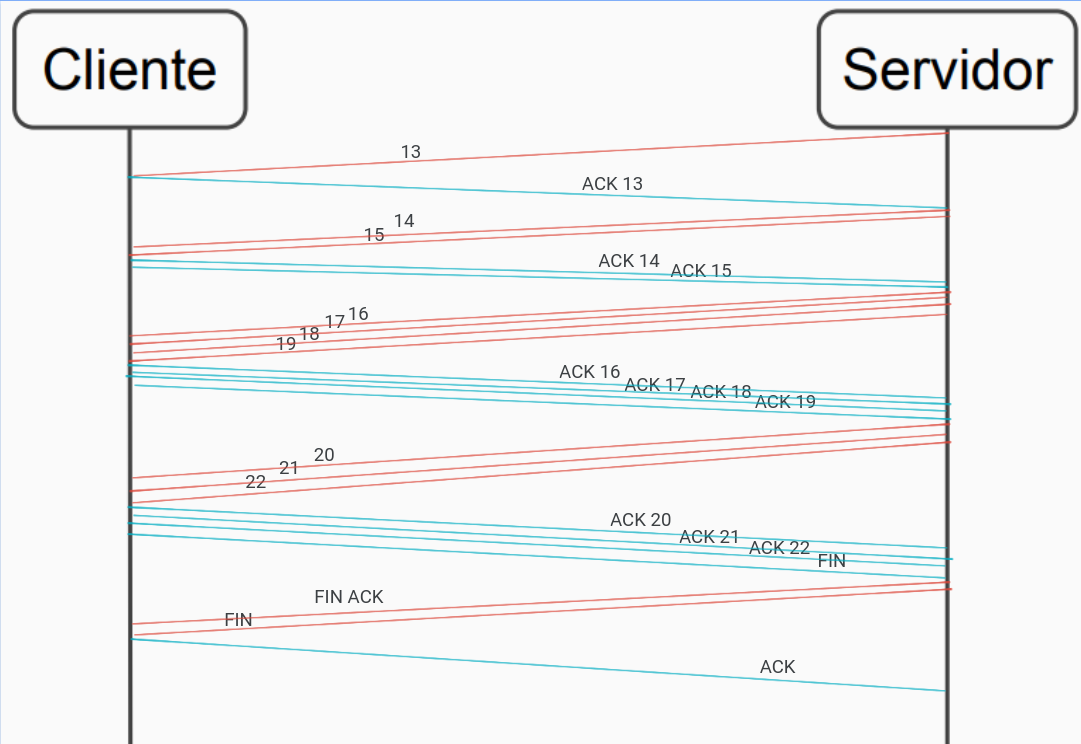
\includegraphics[width=\textwidth]{imagenes/resEj13.png}
\end{figure}

\subsubsection{Ejercicio 2}
Por medio de una conexión TCP se transfiere desde un host A a un host B un archivo de 27326 B. De acuerdo con las tecnologías de enlace que utiliza el host A, MSS=1500B. Además, sabemos que su sistema operativo opera con TCP Tahoe, con una IW=1MSS. El sistema utiliza ssthresh=4MSS. Sabemos que la conexión sufrirá la pérdida del séptimo segmento de datos transmitido.

\subsubsection{Ejercicio 3}

Considere el efecto de usar Slow Start en una conexión TCP recién establecida (IW = 2 * SMSS, SSTHRESH = 64KB), que tiene un RTT de 10 mseg y sin congestión ni errores presentes en la red. La RWND es de 24KB y el SMSS es de 2KB. ¿Cuánto tiempo transcurre antes de que pueda ser enviada la primera ventana de recepción llena? (Asumir que el Ttx de una ventana es una componente despreciable del Delay total de la conexión)


\begin{center}
    \begin{tabular}{c|c|c|c}
        RTT & CWND & RWND & FlightSize \\
        \hline
        \hline
        1 & & & \\
         \hline
        2 & & & \\
         \hline
        3 & & & \\
         \hline
        4 & & & \\
         \hline
        5 & & & \\
         \hline
        6 & & & \\
         \hline
        7 & & & \\
         \hline
        8 & & & \\
         \hline
        9 & & & \\
         \hline
        10 & & & \\
    \end{tabular}
\end{center}


\subsubsection{Ejercicio 4 - Reno}

Por medio de una conexión TCP se transfiere desde un host A a un host B un archivo de 41326 B. De acuerdo con las tecnologías de enlace que utiliza el host A, MSS=2000B. Además, sabemos que su sistema operativo opera con TCP Reno, con una IW=2MSS. El sistema utiliza ssthresh=8MSS. Sabemos que la conexión sufrirá la pérdida del décimo segmento de datos transmitido.

\section{Fragmentacion}\label{sec:fragmentacion}

\subsection{MTU}

Máximo tamaño de paquete de datos que se puede transferir en IP. Depende de la capa de enlace, por lo que no se tiene la misma MTU en Ethernet que en Wi-Fi. El problema surge cuando se quieren enviar paquetes cuyo tamaño es mayor al MTU.

$$ \mathrm{MTU} = \mathrm{MSS} + \mathrm{IP}_{\mathrm{header}} + \mathrm{TCP}_{\mathrm{header}} $$

Para solucionarlo, se fragmenta el datagrama en partes, donde cada fragmento se transmite en un paquete IP diferente. El proceso de fragmentación puede darse tanto en hosts como en routers. Sin embargo, el ensamble solo se realiza en el destino. IP es sin conexion, lo paquetes son tratados individualmente. La informacion para el ensamblado viaja en el header de IP: fragment offset y flags. No pueden llegar sin ensamblar a TCP/UDP. En caso de que uno o más no lleguen, se descarta toda la secuencia.

Los flags pueden ser tres:

\begin{itemize}
    \item [X]: reservado, no se usa
    \item [D]: Do no fragment. Indica si se puede fragmentar o no
    \item [M]: More Fragments. Indica si es el ultimo fragmento o hay más
\end{itemize}

El fragment Offset tiene 3 bits menos que el Total Lenght debido a los flags. Además, cuenta en unidades de 8 bytes. De esta manera, cada bit que nos movemos en el fragment offset implica moverse 8 bits en el total lenght

\begin{center}
    \begin{tabular}{c|c|c|c}
    \hline
         X(1) & D(1) & M(1) & Fragment offset (13)  \\
    \hline     
    \end{tabular}
\end{center}

\textbf{Ejemplo} \\

Suponiendo $ \mathrm{MTU} = 550 B = 530 B_{\mathrm{payload}} + 20 B_{\mathrm{header}} $

Se quiere envian un payload de 800 B. El máximo payload a enviar por paquete es 530. Entonces será un paquete de 530 bytes y otro de 270 bytes.

$$\mathrm{Fragmento}_1 = 530 B$$
$$\mathrm{Fragmento}_2 = 270 B$$

Calculemos el fragment offset de cada uno.

$$ \mathrm{FragmenOffset}_1 = 0 $$
$$ \mathrm{FragmenOffset}_2 =  ? $$

\begin{center}
    \begin{tabular}{c|c}
        Offset Real & Fragment Offset \\
        \hline
        \hline
        8 Bytes & 1 \\
        \hline
        530 Bytes & \textbf{66.25}
    \end{tabular}
\end{center}

66.25 no puede ser expresado en número binario, por lo que hay que cambiar el tamaño de los fragmentos. Para calcular el nuevo tamaño se usa la siguiente fórmula:

$$ \mathrm{FragmentPayloadSize} = \mathrm{floor}(\frac{\mathrm{MaxPayloadSize}}{8}) \cdot 8 $$

En nuestro caso $\mathrm{floor}(\frac{\mathrm{530 B}}{8}) \cdot 8 = 528 B$

$$\mathrm{Fragmento}_1 = 528 B$$
$$\mathrm{Fragmento}_2 = 272 B$$

\begin{center}
    \begin{tabular}{c|c}
        Offset Real & Fragment Offset \\
        \hline
        \hline
        8 Bytes & 1 \\
        \hline
        528 Bytes & \textbf{66}
    \end{tabular}
\end{center}


\subsection{Ejercicio de Parcial}

\subsubsection{Ejercicio 1}
El host A quiere enviar un paquete de tamaño total 620 bytes al host B. El valor del flag Do not fragment es cero.

\begin{figure}[H]
\centering
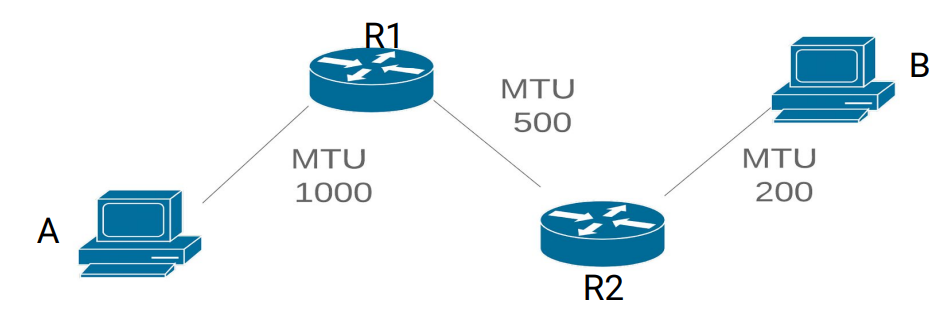
\includegraphics[width=\textwidth]{imagenes/frag1.png}
\end{figure}

\textbf{A - R1}\\
En la conexion del host a con R1 se comprueba que el MTU es mayor al paquete que desea envíar. Por lo que se envia el paquete sin fragmentacion

$$ \mathrm{MTU} = 1000 $$
$$ \mathrm{Paquete} = 620 $$
$$ \mathrm{MTU}  \geq \mathrm{Paquete}$$

\begin{itemize}
    \item Total Lenght: 620 bytes
    \item X: reservado
    \item D: 0
    \item M: 0
    \item Fragment Offset: 0
\end{itemize}


\textbf{R1 - R2}\\

En la conexión de R1 con R2 se verifica que el MTU es menor a el paquete a enviar, además el Do Not Fragment es cero por lo que debe fragmentarse el paquete.

$$ \mathrm{MTU} = 500 $$
$$ \mathrm{Paquete} = 620 $$
$$ \mathrm{MTU}  \le \mathrm{Paquete}$$

El MTU incluye al header, asumo que es de 20 Bytes. Entonces en máximo tamaño de payload será de 480 Bytes

$$ \mathrm{MaxPayloadSize} = \mathrm{MTU} - \mathrm{Lenght}(\mathrm{Header}) = 500 - 20 = 480 $$

$$\mathrm{floor}(\frac{\mathrm{480 B}}{8}) \cdot 8 = 480 B$$

De esta manera se van a enviar 2 fragmentos:

\textbf{Recordar no tener en cuenta el header del mensaje original.}


$$ \mathrm{PayloadOriginal} = 620 - 20 = 600 $$
$$\mathrm{Fragmento}_1 = 480 B$$
\begin{itemize}
    \item Total Lenght: 480 + 20 bytes
    \item X: reservado
    \item D: 0
    \item M: 1
    \item Fragment Offset: 0
\end{itemize}

$$\mathrm{Fragmento}_2 = 600 - 480 = 120 B$$

\begin{center}
    \begin{tabular}{c|c}
        Offset Real & Fragment Offset \\
        \hline
        \hline
        8 Bytes & 1 \\
        \hline
        480 Bytes & \textbf{60}
    \end{tabular}
\end{center}

\begin{itemize}
    \item Total Lenght: 120 + 20 bytes
    \item X: reservado
    \item D: 0
    \item M: 0
    \item Fragment Offset: 60
\end{itemize}


\textbf{R2 - RB}\\

Para el primer fragmento, el MTU es menor al tamaño, por lo que habrá que fragmentar. El Largo total del segundo fragmento puede reenviarse sin fragmentar.


$$ \mathrm{MTU} = 200 $$
$$ \mathrm{Fragmento}_1 = 500 $$

$$ \mathrm{MaxPayloadSize} = \mathrm{MTU} - \mathrm{Lenght}(\mathrm{Header}) = 200 - 20 = 180 $$

$$ \mathrm{FragmentPayloadSize} = \mathrm{floor}(\frac{\mathrm{MaxPayloadSize}}{8}) \cdot 8 = \mathrm{floor}(\frac{\mathrm{180}}{8}) \cdot 8  = 176 $$

Recordar de que el payload del fragmento 1 es de 480. Entonces se enviarán dos fragmentos de 176 y uno de 128

\begin{center}
    \begin{tabular}{c|c}
        Offset Real & Fragment Offset \\
        \hline
        \hline
        8 Bytes & 1 \\
        \hline
        176 Bytes & \textbf{22} \\
        \hline
        352 Bytes & \textbf{44}
    \end{tabular}
\end{center}

\begin{center}
    \begin{tabular}{c|c|c|c|c|c}
    Fragmento & Total Lenght & X & D & M & Fragment Offset \\
        \hline
        \hline
    $ \mathrm{Fragmento}_{1_1} $  &  176 + 20  & X & 0 & 1 & 0   \\
    \hline
    $ \mathrm{Fragmento}_{1_2} $  &  176 + 20  & X & 0 & 1 & 22 \\
    \hline
    $ \mathrm{Fragmento}_{1_3} $ &  128 + 20  & X & 0 & 1 & 44 \\
    \hline
    $ \mathrm{Fragmento}_{2} $  & 120 + 20 & X & 0 & 0 & 60
    \end{tabular}
\end{center}

La suma de los payloads, da un payload total de 600 que es el payload que se tenia originalmente (más 20 de header)

\subsubsection{Ejercicio 2}


El host A envia un datagrama IP cuyo payload es 1480 Bytes.

\begin{figure}[H]
\centering
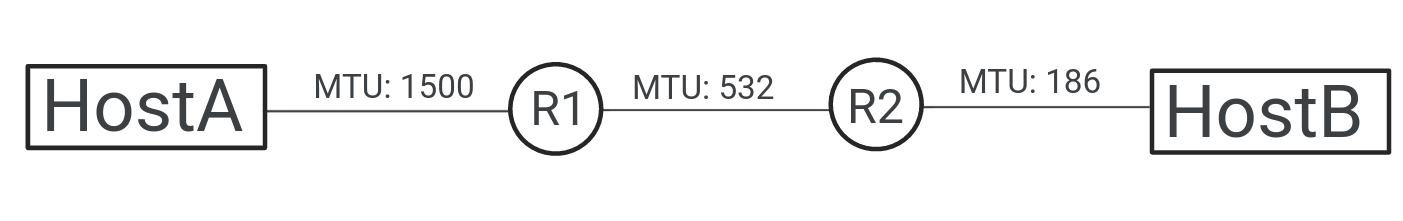
\includegraphics[width=\textwidth]{imagenes/enunciadoFragmentacion.png}
\end{figure}


El paquete es de 1500 bytes (1480 + 20 del header). En el primer traspaso, alcanza el MTU.

$$ \mathrm{MaxPayloadSize} = MTU - \mathrm{Lenght}(\mathrm{Header}) = 1500 - 20 = 1480 $$
$$\mathrm{floor}(\frac{\mathrm{1480 B}}{8}) \cdot 8 = 185 B$$

No es necesario fragmentar en este primer tramo.

En el tramo del primer al segundo router hay que fragmentar, ya que el MTU es menor al tamaño del paquete. Se calcula el máximo payload para este tramo:

$$ \mathrm{MaxPayloadSize} = MTU - \mathrm{Lenght}(\mathrm{Header}) = 532 - 20 = 502 $$

$$\mathrm{floor}(\frac{\mathrm{502 B}}{8}) \cdot 8 = 496 B$$

\begin{center}
    \begin{tabular}{c|c|c|c}
        Fragmento & Total Lenght & Fragment Offset & More Fragments \\
        \hline
        \hline
        $ \mathrm{Fragmento}_1 $ & 496 + 20  & 0 & 1\\
        $ \mathrm{Fragmento}_2 $ &  496 + 20 & 62 & 1\\
        $ \mathrm{Fragmento}_3 $ & 488 + 20 & 124 & 0\\
    \end{tabular}
\end{center}

Para el tramo del segunto router al Host B habrá que fragmentar todos ya que el MTU es más chico.

$$ \mathrm{MaxPayloadSize} = MTU - \mathrm{Lenght}(\mathrm{Header}) = 186 - 20 = 166 $$

$$\mathrm{floor}(\frac{\mathrm{166 B}}{8}) \cdot 8 = 160 B$$



\begin{center}
    \begin{tabular}{c|c|c|c}
        Fragmento & Total Lenght & Fragment Offset & More Fragments \\
        \hline
        \hline
        $ \mathrm{Fragmento}_{11} $ & 160 + 20  & 0 & 1\\
        \hline
        $ \mathrm{Fragmento}_{12} $ & 160 + 20  & 20 & 1\\
        \hline
        $ \mathrm{Fragmento}_{13} $ & 160 + 20  & 40 & 1\\
        \hline
        $ \mathrm{Fragmento}_{14} $ & 16 + 20  & 60 & 1\\
        \hline
        \hline
        \hline
        $ \mathrm{Fragmento}_{21} $ & 160 + 20  & 62 & 1\\
        \hline
        $ \mathrm{Fragmento}_{22} $ & 160 + 20  & 82 & 1\\
        \hline
        $ \mathrm{Fragmento}_{23} $ & 160 + 20  & 102 & 1\\
        \hline
        $ \mathrm{Fragmento}_{24} $ & 16 + 20  & 122 & 1\\
        \hline
        \hline
        \hline
        $ \mathrm{Fragmento}_{31} $ & 160 + 20  & 124 & 1\\
        \hline
        $ \mathrm{Fragmento}_{32} $ & 160 + 20  & 144 & 1\\
        \hline
        $ \mathrm{Fragmento}_{33} $ & 160 + 20  & 164 & 1\\
        \hline
        $ \mathrm{Fragmento}_{34} $ & 8 + 20  & 184 & 0\\
    \end{tabular}
\end{center}

Se puede verificar ya que el fragment offset total de la segunda tabla es $124 + \frac{488}{8} = 185$ y el fragment offset total de la última tabla es $184 + \frac{8}{8} = 185$. 
Además si se suman los payloads se llega a un total de 1480, igual al payload del mensaje original.




\section{Subnetting}\label{sec:subnetting}

\subsection{Arquitectura de clases Ip}

Al principio las direcciones se interpretaban como 8 bits para la direccion de red y 24 para la dirección del host: \textcolor{red}{154}.\textcolor{blue}{200}.\textcolor{blue}{31}.\textcolor{blue}{1}

Luego se introduce el \textbf{Classful  Addresing} para dividir el espacion de direcciones en clases:

\begin{itemize}
    \item Clase A: \textcolor{red}{10}.\textcolor{blue}{20}.\textcolor{blue}{0}.\textcolor{blue}{7}
    \item Clase B: \textcolor{red}{154}.\textcolor{red}{13}.\textcolor{blue}{22}.\textcolor{blue}{3}
    \item Clase C: \textcolor{red}{200}.\textcolor{red}{4}.\textcolor{red}{67}.\textcolor{blue}{3}
    \item Clase D: Multicast
    \item Clase E: Experimental
\end{itemize}

Posteriormente se introduce \textbf{e Classless Inter-Domain Routing (CIDR)} que implica máscaras de subred de longitud variable: 200.4.67.3 \textcolor{yellow}{/23}

\subsection{Subnets}

Una subnet es una subdivision lógica de una red, permitiendo agrupar direcciones en un rango. Se describen por ejemplo: 192.168.1.0/24.
La máscara permite reducir la lógica que tienen que manejar los routers, permitiendo separar el tráfico en subredes optimizando el uso de la red. A su vez reduciendo la congestion de red, aumentando la seguridad y facilitando la administracion de la red.

\subsection{Ejercicios}

En los ejercicios de subnetting, dada una subred se busca maximizar la cantidad de direcciones ocupada ya que cada direccion inactiva desperciada es plata tirada.

\subsubsection{Metodologia}
Todas las subredes tienen una direccion de red y una direccion de broadcast. No se puede asignar la direccion de red o la de broadcast a un host. Todos los dispositivos conectados a la red tienen una dirección IP (los routers también).

$$ \mathrm{\# de hosts} = 2^{32-\mathrm{mascara}}-2 $$ 

El último 2 restando se debe a que las direcciones de red y broadcast no se pueden usar

\subsection{Ejercicio 1}

\begin{figure}[H]
\centering
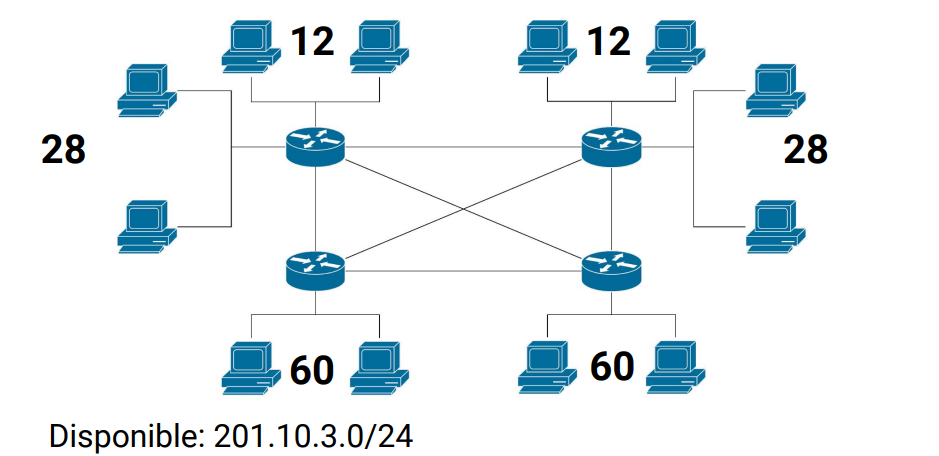
\includegraphics[width=\textwidth]{imagenes/enunciado1subnetting.png}
\end{figure}

A priori se pueden identificar 6 subredes (cada una con la cantidad de hosts), 4 routers y 6 enlaces entre routers. Hay que tener en cuenta que \textcolor{red}{los enlaces punto a punto entre routers necesitan tener su propia subred}. De esta manera, quedan 12 subredes, 4 routers y 6 enlaces entre routers. Ademas \textcolor{red}{201}.\textcolor{red}{10}.\textcolor{red}{3}.\textcolor{blue}{0}. Entonces se tienen 8 bits para las direcciones de host, es decir 256 direcciones

\begin{figure}[H]
\centering
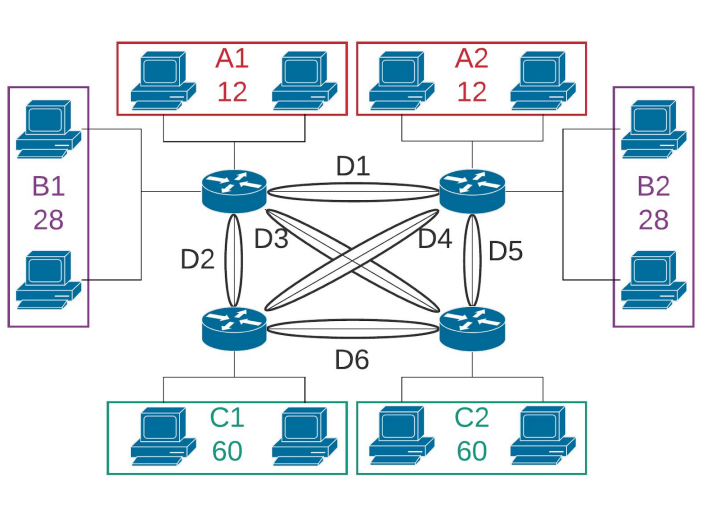
\includegraphics[width=\textwidth]{imagenes/subnetting12.png}
\end{figure}

Para delimitar las subredes:

\begin{itemize}
    \item Ver cuantos hosts tiene cada uno (sin olvidar los routers)
    \item Averiguar el espacio de direcciones a subdividir
    \item asignar la minima cantidad de IP a cada subred
\end{itemize}

Las redes con más hosts son \textbf{C1} y \textbf{C2} con 60 hosts más un router cada una. Como las 256 direcciones disponibles son mayores a las 61 que precisa la red, se divide en 2 la red. Se tienen 2 redes /25 con 128 direcciones cada una.

\begin{figure}[H]
\centering
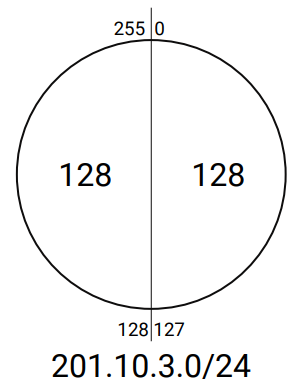
\includegraphics[width=0.3\textwidth]{imagenes/subnetting13.png}
\end{figure}


\begin{figure}[H]
\centering
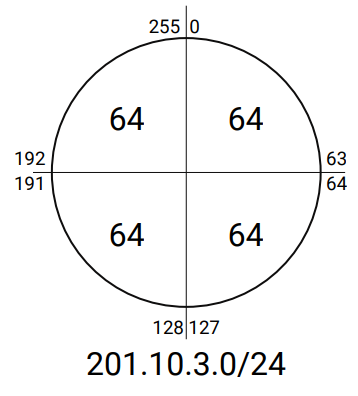
\includegraphics[width=0.3\textwidth]{imagenes/subnetting14.png}
\end{figure}


Sin embargo sigue siendo muy mayor 128 a 61, entonces se divide la red nuevamente. Se tienen 4 redes /26 con 64 direcciones cada una. Si dividiera nuevamente, quedarian redes con 32 direcciones, insuficientes para C1 y C2. Entonces asigno a C1 y a C2 a cada espacio de 64 direcciones

\begin{figure}[H]
\centering
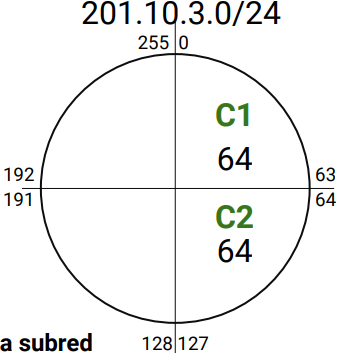
\includegraphics[width=0.3\textwidth]{imagenes/subnetting15.png}
\end{figure}

De esta manera, las direcciones de las subredes quedarian asignadas de la siguiente manera:

\begin{center}
    \begin{tabular}{c|c}
    Subred & Dirección de la subred \\
    \hline
    \hline
    C1     & 201.10.3.0 / 26 \\
    C2     & 201.10.3.64 / 26
    \end{tabular}
\end{center}


Las redes siguientes en tamaño son B1 y B2 con 28 hosts cada una. Quedan 2 redes de 64, puede dividirse una y quedan de 32 para asignar.


\begin{center}
    \begin{tabular}{c|c}
    Subred & Dirección de la subred \\
    \hline
    \hline
    C1     & 201.10.3.0 / 26 \\
    C2     & 201.10.3.64 / 26 \\
    B1     201.10.3.128 / 27 \\
    B2     & 201.10.3.160 / 27
    \end{tabular}
\end{center}


\begin{figure}[H]
\centering
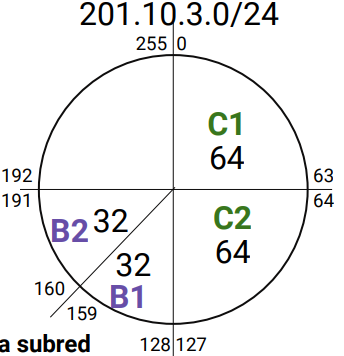
\includegraphics[width=0.3\textwidth]{imagenes/subnetting16.png}
\end{figure}

Se procede de igual manera con las redes que siguen en cantidad de hosts


\begin{center}
    \begin{tabular}{c|c}
    Subred & Dirección de la subred \\
    \hline
    \hline
    C1     & 201.10.3.0 / 26 \\
    \hline
    C2     & 201.10.3.64 / 26 \\
    \hline
    B1     & 201.10.3.128 / 27 \\
    \hline
    B2     & 201.10.3.160 / 27 \\
    \hline
    A1     & 201.10.3.192 / 28 \\
    \hline
    A2     & 201.10.3.208 / 28 \\
    \hline
    D1     & 201.10.3.224 / 30\\
    \hline
    D2     & 201.10.3.228 / 30 \\
    \hline
    D3     & 201.10.3.232 / 30 \\
    \hline
    D4     & 201.10.3.236 / 30\\
    \hline
    D5     & 201.10.3.240 / 30 \\
    \hline
    D6     & 201.10.3.244 / 30 \\
    \end{tabular}
\end{center}


\begin{figure}[H]
\centering
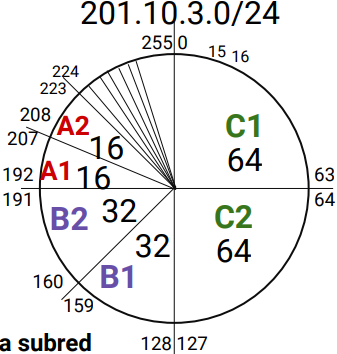
\includegraphics[width=0.3\textwidth]{imagenes/subnetting17.png}
\end{figure}


\subsection{Ejercicio 2}

Dada la siguiente configuración de hosts y routers, y el espacio 192.168.0.0/23, se pide separar en subredes minimizando la cantidad de IPs sin usar. Ante igualdad de condiciones para ubicar varias subredes:
\begin{itemize}
    \item Asignar bloques utilizando los prefijos en orden de numeración ascendente (Ej: si tenemos la opcion de usar 117.0.1.0/24 o 117.0.0.0/24, debemos utilizar primero el espacio de direcciones 117.0.0.0/24).
    \item  Asignar bloques de direcciones priorizando las redes con mayor cantidad de hosts (Ej: si se deben asignar dos bloques de 64 direcciones IP para dos subredes distintas Sx y Sy , donde x e y representan la cantidad de hosts de cada subred y con 32 < x < y < 64, Sy debe asignarse en un espacio de direcciones de menor numeración).
    \item Si dos subredes necesitan la misma cantidad de IPs, ubicar primero la subred cuya letra viene primero en el abecedario (Ej: si las redes P y J tienen necesitan un bloque de 32 IPs, ubicar primero la J y luego la P).
\end{itemize}
Este criterio arbitrario define una única resolución posible de la configuración. Cualquier otra solución será considerada incorrecta.

\begin{figure}[H]
\centering
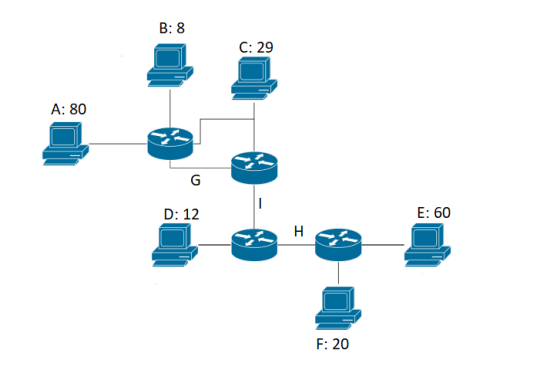
\includegraphics[width=\textwidth]{imagenes/subnetting2.png}
\end{figure}


\section{Teoria}\label{sec:teoria}


\subsection{Capa de Aplicación}\label{sec:capaaplicacion}

Los protocolos de la capa de aplicación se implementan en los hosts


\subsection{Protocolo\label{sec:protocolo}}


\subsubsection{ ¿Cuál es la función de un protocolo de capa de aplicación?}

La función de un protocolo de la capa de aplicación es la de ...

\subsubsection{¿Qué define un protocolo?} 
Conjunto definido de reglas y procedimientos que determinan cómo se transmiten los datos en las redes de computadoras. Un protocolo define:

\begin{itemize}
    \item Mensajes de petición y respuesta
    \item Sintaxis de los mensajes
    \item Campos - función, tamaño y delimitadores
    \item Procedimiento de envío de mensajes y sus respuestas
\end{itemize}

\subsection{PING}

Se utiliza para comprobar el tiempo que tarda un paquete de información en llegar a una dirección IP que se haya indicado y luego volver. PING puede enviar 2 paquetes:

\begin{itemize}
    \item ICMP Echo Request
    \item ICMP Echo Replay/Response
\end{itemize}

Esto permite diagnosticar el estado, velocidad y calidad de una red

\subsection{ICMP}

Es un protocolo de señales para IP. Incluye mensajes de control, diagnostico y reporte de errores. Tiene 2 categorías importantes de mensajes:
\begin{itemize}
    \item Query
    \item Error reporting
\end{itemize}


\end{document}
